\chapter{曲率的序言}
\label{chap5}

\begin{align}
    1\\2
\end{align}

\section{引力与曲率的关系}
\label{sec5.1}
前面都是在狭义相对论(SR)中讨论问题。力在SR当中的地位很重要,但是前面从来没有直接研究引力。SR的一个重要基础是存在覆盖整个时空的惯性系:全体时空可以由一个坐标系描述,这个系的所有坐标点总是相对于原点静止,所有的坐标钟与原点的钟走时率相同。从这个基本假设可以导出时间间隔$\Delta s^2$的概念,它给物理事件赋予了具有不变性的几何意义。例如,两事件之间的类时间隔是经过这两个时件的钟所走过的时间;类空间隔是在这两个事件同时的坐标系当中的空间距离。

度规是计算间隔的数学函数,因此SR的度规是由杆的长度和钟的走时定义的。  This is the power of SR and one reason for the elegance and compactness of tensor notation in it (例如用$\vec{N}$统一表示了“数密度”和“流量”)。

(未完成)

\section{极坐标系的张量代数}
\label{sec5.2}
考虑欧几里得平面。直角坐标$\{x, y\}$,极坐标$\{r, \theta\}$之间的关系为:
\begin{equation}
    \left.
    \begin{split}
    r &= (x^2 + y^2)^{1/2}, \quad x = r \cos \theta, \\
    \theta &= \Arctan (y / x), \quad y = r \sin \theta.
    \end{split}
    \right\}
\label{equ5.3}
\end{equation}

由直角坐标的微小增量$\Delta x, \Delta y$造成的$\Delta r, \Delta \theta$为
\begin{equation}
\left.
\begin{split}
    \Delta r &= \frac{x}{r} \Delta x + \frac{y}{r} \Delta y = \cos \theta \Delta x + \sin \theta \Delta y, \\
    \Delta \theta &= -\frac{y}{r^2} \Delta x + \frac{x}{r^2} \Delta y = -\frac{1}{r} \sin \theta \Delta x + \frac{1}{r} \cos \theta \Delta y,
\end{split}
\right\}
\label{equ5.4}
\end{equation}
上式到一阶小量都成立。

也可以使用其它坐标系。记一般的坐标系为$\{ \xi, \eta \}$:
\begin{equation}
\left.
\begin{split}
    \xi &= \xi (x, y), \quad \Delta \xi = \frac{\partial \xi}{\partial x} \Delta x + \frac{\partial \xi}{\partial y} \Delta y, \\
    \eta &= \eta (x, y), \quad \Delta \eta = \frac{\partial \eta}{\partial x} \Delta x + \frac{\partial \eta}{\partial y} \Delta y.
\end{split}
\right\}
\label{equ5.5}
\end{equation}
为了保证$(\xi, \eta)$是个好坐标系,任意两个不同的点$(x_1, y_1)$和$(x_2, y_2)$应该对应不同的$(\xi_1, \eta_1)$与$(\xi_2, \eta_2)$(通过\eqref{equ5.5}式对应)。例如,按$\xi = x, \eta = 1$定义的坐标系不是好坐标系,因为不同的两点$(x = 1, y = 2)$和$(x = 1, y = 3)$都对应$(\xi = 1, \eta = 1)$。数学上,这要求如果方程\eqref{equ5.5}中的$\Delta \xi = \Delta \eta = 0$,则必须对应相同的点,即$\Delta x = \Delta y = 0$. 这意味着\eqref{equ5.5}式的行列式非零:
\begin{equation}
    \det \begin{pmatrix}
        \partial \xi / \partial x & \partial \xi / \partial y \\
        \partial \eta / \partial x & \partial \eta / \partial y
    \end{pmatrix} 
    \neq 0.
\label{equ5.6}
\end{equation}
这个行列式称为坐标系变换\eqref{equ5.5}式的\textit{Jacobian}(\textit{雅可比行列式})。如果Jacobian在某一点为零,则称坐标变换在该点具有\textit{奇性 (singular)}。

\subsection*{向量与1形式}
向量的旧的定义是在\textit{任意}坐标变换下与位移的变换方式相同的量。也就是说,向量$\Delta \vec{r}$可以表示为\footnote{欧几里得空间的向量用箭头标记,其分量指标(1, 2)用希腊字母表示,求和对所有指标进行。}位移$(\Delta x, \Delta y)$,或者在极坐标系表示为$(\Delta r, \Delta \theta)$,或者在一般坐标系中为$(\Delta \xi, \Delta \eta)$. 根据\eqref{equ5.5}式,对于微小的$(\Delta x, \Delta y)$有:
\begin{equation}
    \begin{pmatrix}
        \Delta \xi \\ \Delta \eta
    \end{pmatrix}
    =
    \begin{pmatrix}
        \partial \xi / \partial x & \partial \xi / \partial y \\
        \partial \eta / \partial x & \partial \eta / \partial y 
    \end{pmatrix}
    \begin{pmatrix}
        \Delta x \\ \Delta y 
    \end{pmatrix}.
\label{equ5.7}
\end{equation}
定义变换矩阵
\begin{equation}
    (\Lambda\indices{^{\alpha'}_{\beta}}) = 
    \begin{pmatrix}
        \partial \xi / \partial x & \partial \xi / \partial y \\
        \partial \eta / \partial x & \partial \eta / \partial y 
    \end{pmatrix},
\label{equ5.8}
\end{equation}
则可以将任意向量$\vec{V}$的分量的变换规律写成与SR相同的形式:
\begin{equation}
    V^{\alpha'} = \Lambda\indices{^{\alpha'}_{\beta}} V^\beta,
\label{equ5.9}
\end{equation}
其中不带撇的指标代表$(x, y)$,带撇指标表示$(\xi, \eta)$,指标取$1, 2$. 向量可以定义为分量按照\eqref{equ5.9}式变换的这样的量。不过,存在一种更加复杂而自然的、现代的定义方式,下面进行介绍。

考虑平面上的标量场$\phi$。给定坐标系$(\xi, \eta)$就能计算偏导数$\partial \phi / \partial \xi$和$\partial \phi / \partial \eta$. \textit{定义}1形式$\trd \phi$为(在坐标系$(\xi, \eta)$中)具有如下分量的几何对象:
\begin{equation}
    \trd \phi \to (\partial \phi / \partial \xi, \partial \phi / \partial \eta).
\label{equ5.10}
\end{equation}
这是1形式的一般定义,每个标量场都定义了一个1形式。1形式分量的变换规律可以通过链式法则(chain rule)导出:
\begin{equation}
    \frac{\partial \phi}{\partial \xi} = \frac{\partial x}{\partial \xi} \frac{\partial \phi}{\partial x} + \frac{\partial y}{\partial \xi} \frac{\partial \phi}{\partial y},
\label{equ5.11}
\end{equation}
$\partial \phi / \partial \eta$同理。用\textit{行向量}可以方便地用矩阵形式表示:
\begin{equation}
\begin{pmatrix}
    \partial \phi / \partial \xi & \partial \phi / \partial \eta
\end{pmatrix}
=
\begin{pmatrix}
    \partial \phi / \partial x & \partial \phi / \partial y
\end{pmatrix}
\begin{pmatrix}
    \partial x / \partial \xi & \partial x / \partial \eta \\
    \partial y / \partial \xi & \partial y / \partial \eta
\end{pmatrix},
\label{equ5.12}
\end{equation}

1形式的变换矩阵可类比\eqref{equ5.8}式定义为一组$(x, y)$坐标关于$(\xi, \eta)$坐标的偏导数:
\begin{equation}
    ( \Lambda\indices{^\alpha_{\beta'}} ) = 
    \begin{pmatrix}
        \partial x / \partial \xi & \partial x / \partial \eta \\
        \partial y / \partial \xi & \partial y / \partial \eta
    \end{pmatrix}
\label{equ5.13}
\end{equation}
这样,\eqref{equ5.12}式就可以写成分量求和的形式:
\begin{equation}
    (\trd \phi)_{\beta'} = \Lambda\indices{^\alpha_{\beta'}} (\trd \phi)_\alpha.
\label{equ5.14}
\end{equation}
注意,上式的求和是对变换矩阵的\textit{第一个}分量进行的,这对应于行向量左乘矩阵。

值得一提的是,SR从来没考虑过行向量,因为Lorentz变换矩阵是个简单的对称矩阵。不过即使是上面的简单情况也要用到行向量。当张量的指标多于两个时,矩阵表示就非常累赘。GR需要处理四个甚至五个指标的张量,因此后面一般用代数形式(如\eqref{equ5.14}式)表示变换,后面就不再使用矩阵表示了。

本节已经看到,在现代观点之下,张量代数的基础是1形式的定义。它比旧定义更加自然,旧定义首先定义了\textit{单个}向量$(\Delta x, \Delta y)$,其它向量类比它定义。而现代定义利用偏导数定义了\textit{一类}1形式,1形式分量的变换规律自然地随之导出。

向量定义为将1形式映射为实数的线性函数。这个定义的具体含义在下一小节讲述。先来说明与SR形式的相似性,向量的变换规律为$\eqref{equ5.9}$式,有趣的是变换矩阵$(\Lambda\indices{^{\alpha'}_\beta})$和$( \Lambda\indices{^\alpha_{\beta'}} )$互逆。它们相乘得到:
\begin{align}
    \begin{pmatrix}
        \partial \xi / \partial x & \partial \xi / \partial y \\
        \partial \eta / \partial x & \partial \eta / \partial y 
    \end{pmatrix}
    \begin{pmatrix}
        \partial x / \partial \xi & \partial x / \partial \eta \\
        \partial y / \partial \xi & \partial y / \partial \eta
    \end{pmatrix} \notag \\
    =
    \begin{pmatrix}
        \dfrac{\partial \xi}{\partial x} \dfrac{\partial x}{\partial \xi} + \dfrac{\partial \xi}{\partial y} \dfrac{\partial y}{\partial \xi} & \dfrac{\partial \xi}{\partial x} \dfrac{\partial x}{\partial \eta} + \dfrac{\partial \xi}{\partial y} \dfrac{\partial y}{\partial \eta}  \\
        \dfrac{\partial \eta}{\partial x} \dfrac{\partial x}{\partial \xi} + \dfrac{\partial \eta}{\partial y} \dfrac{\partial y}{\partial \xi} & \dfrac{\partial \eta}{\partial x} \dfrac{\partial x}{\partial \eta} + \dfrac{\partial \eta}{\partial y} \dfrac{\partial y}{\partial \eta}
    \end{pmatrix}.
\label{equ5.15}
\end{align}
利用链式法则与偏导数的定义可以算出结果为
\begin{equation}
    \begin{pmatrix}
        \partial \xi / \partial \xi & \partial \xi / \partial \eta \\
        \partial \eta / \partial \xi & \partial \eta / \partial \eta
    \end{pmatrix}
    = 
    \begin{pmatrix}
        1 & 0 \\
        0 & 1
    \end{pmatrix}。
\label{equ5.16}
\end{equation}

\subsection*{曲线与向量}
通常所说的曲线是平面上一系列连续的点,我们把它称作\textit{路径 (path)},而把曲线专指参数化的路径。这也是现代数学的做法,将\textit{曲线 (curve)}定义为从实数区间到平面路径的映射。这意味着曲线是每一点都对应一个实数的路径,实数称为参数(parameter),记作$s$。每一点的坐标表示为参数$s$的函数就定义了平面上的一条曲线:
\begin{shaded}
\begin{equation}
    \text{曲线:} \{ \xi = f(s), \eta = g(s), \quad a \le s \le b \}
\label{equ5.17}
\end{equation}
\end{shaded}
将参数改变为$s' = s'(s)$(新参数是旧参数的函数,点不变),则有
\begin{equation}
    \text{曲线:} \{ \xi = f'(s'), \eta = g'(s'), \quad a' \le s' \le b' \},
\label{equ5.18}
\end{equation}
其中$f', g'$是\textit{新的}函数,而$a' = s'(a), b' = s'(b)$. 上式在数学上是一条\textit{新的}曲线,尽管它的\textit{像 (image)}(所经过的平面上的点)与原来相同。因此同一路径对应无数条曲线。

标量场$\phi$沿曲线的导数是$\rd \phi / \rd s$,依赖于$s$,因此变换参数,导数也随之变换。可以将导数写为
\begin{equation}
    \frac{\rd \phi}{\rd s} = \langle \trd \phi, \vec{V} \rangle,
\label{equ5.19}
\end{equation}
其中$\vec{V}$是分量为$(\rd \xi / \rd s, \rd \eta / \rd s)$的向量,这个向量只与曲线有关,而$\trd \phi$只依赖于$\phi$. 因此$\vec{V}$是与曲线特征有关的向量,称之为\textit{切向量 (tangent vector)}。(见图\ref{fig5.4},显然它与曲线相切) \ \sout{画外音:哪里显然了……}

所以,向量可以看作是给定$\phi$而产生$\rd \phi / \rd s$的东西。这就引出了最现代的观点,曲线的切向量应该\textit{称为} $\rd / \rd s$。有些相对论文献偶尔使用这一符号。不过我们把它记作$\vec{V}$,知道它的分量是$(\rd \xi / \rd s, \rd \eta / \rd s)$就好了。注意,平面上的一条路径上的任一点都有着无数切向量,它们的方向相同而长度不同,它们可以视为\textit{不同}曲线(在一点邻域中的参数化不同)的切向量。曲线是给定了参数的路径,因此曲线的切向量\textit{唯一}。此外,即使两条曲线在某一点的切向量相等,它们在其它点也可以不同,根据Taylor展开式$\xi (s + 1) \approx \xi (s) + \rd \xi / \rd s$可见,$\vec{V} (s)$近似沿曲线从$s$到$s + 1$延展。

{
    \centering
    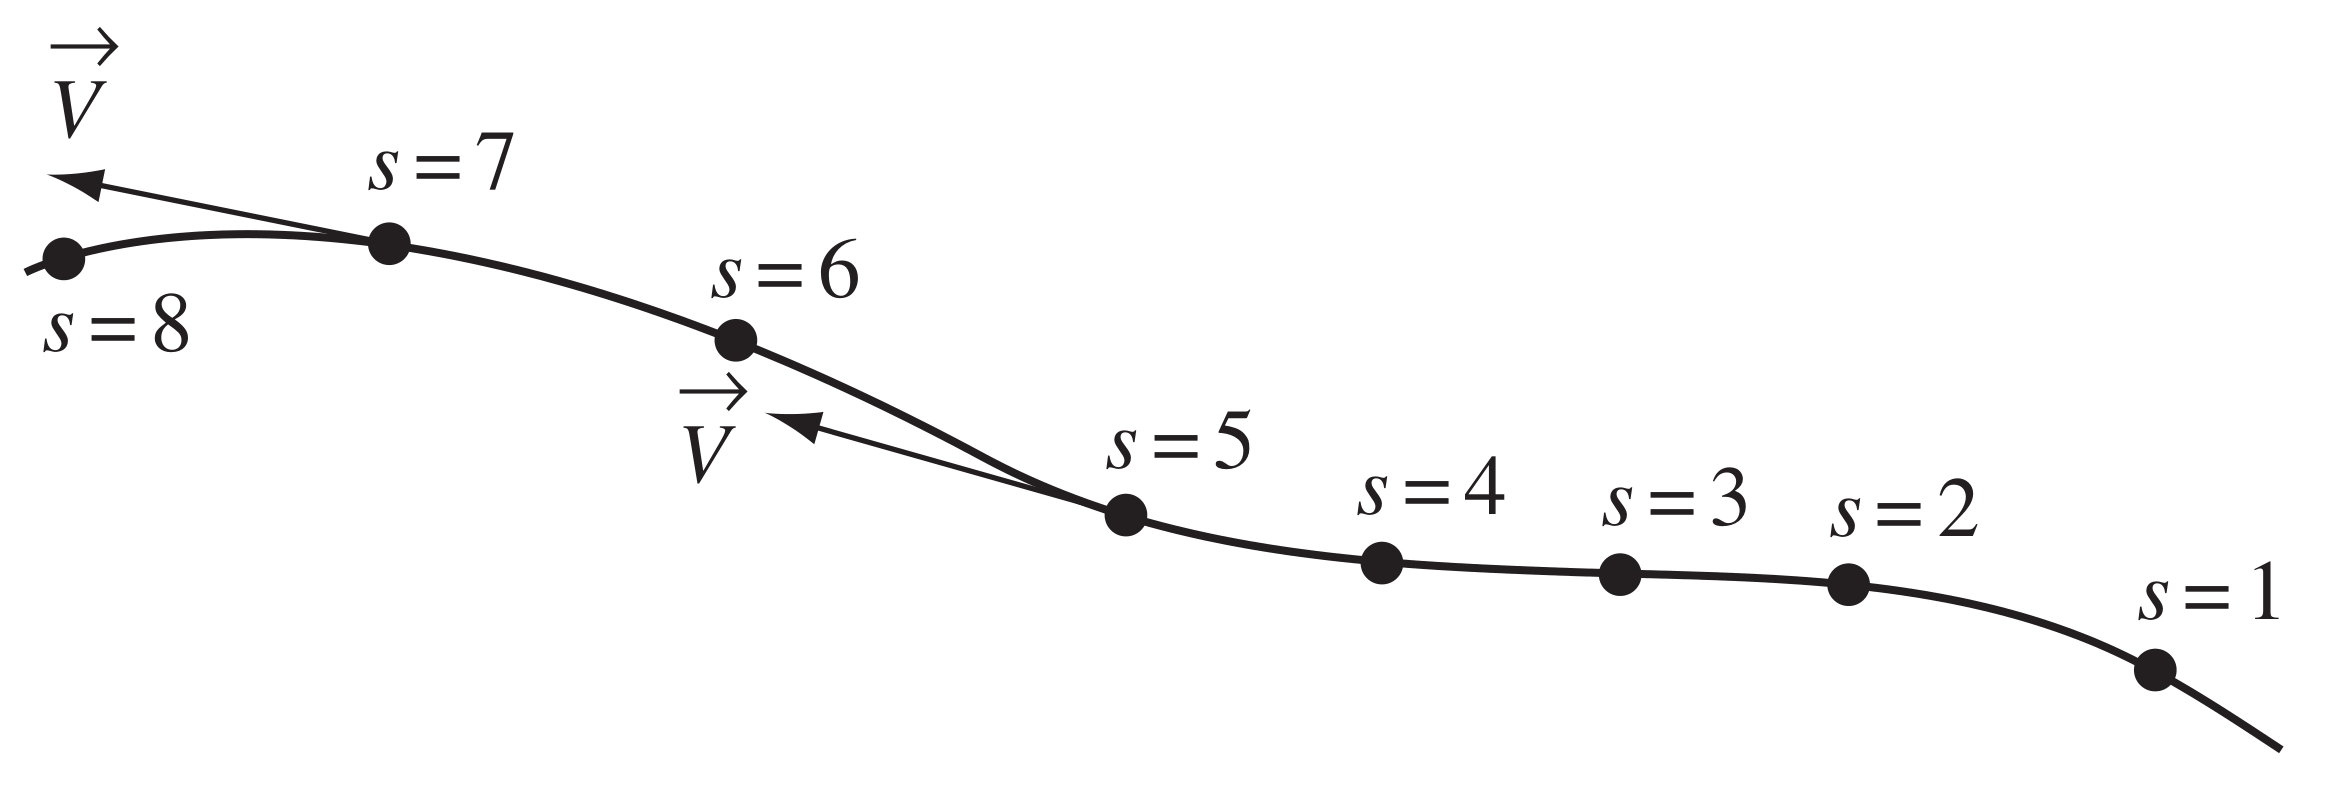
\includegraphics[width=0.6\textwidth]{fig5.4.png}
    \figcaption{\textit{一条曲线,曲线的参数,以及曲线的切向量}}
    \label{fig5.4}
}

注意$s$在坐标变换下不变(它的定义和坐标系无关),而$\vec{V}$的分量变化,因此根据链式法则可得
\begin{equation}
    \begin{pmatrix}
        \rd \xi / \rd s \\
        \rd \eta / \rd s
    \end{pmatrix}
    =
    \begin{pmatrix}
        \partial \xi / \partial x & \partial \xi / \partial y \\
        \partial \eta / \partial x & \partial \eta / \partial y
    \end{pmatrix}
    \begin{pmatrix}
        \rd x / \rd s \\
        \rd y / \rd s
    \end{pmatrix}.
\label{equ5.20}
\end{equation}
这与前面的向量变换律\eqref{equ5.7}式相同。

总结一下现代观点,向量是与某条曲线相切、将$\trd \phi$映射为$\rd \phi / \rd s$的线性函数。这样,下面就能更进一步地研究极坐标系。

\subsection*{极坐标系的1形式基与向量基}
显然,坐标基向量的变换规律为:
\begin{equation*}
    \vec{e}_{\alpha'} = \Lambda\indices{^\beta_{\alpha'}} \vec{e}_\beta,
\end{equation*}
在极坐标下:
\begin{align}
    \vec{e}_r &= \Lambda\indices{^x_r} \Ve_x + \Lambda\indices{^y_r} \Ve_y \label{equ5.21} \\
    &= \frac{\partial x}{\partial r} \Ve_x + \frac{\partial y}{\partial r} \Ve_y \notag \\
    &= \cos \theta \Ve_x + \sin \theta \Ve_y, \label{equ5.22}
\end{align}
类似有
\begin{align}
    \Ve_\theta &= \frac{\partial x}{\partial \theta} \Ve_x + \frac{\partial y}{\partial \theta} \Ve_y \notag \\
    &= -r \sin \theta \Ve_x + r \cos \theta \Ve_y, \label{equ5.23}
\end{align}
注意,上式已经利用了
\begin{equation}
    \Lambda\indices{^x_r} = \frac{\partial x}{\partial r}.
\label{equ5.24}
\end{equation}
类似地,“反向”变换的矩阵元为
\begin{equation}
    \Lambda\indices{^r_x} = \frac{\partial r}{\partial x}.
\label{equ5.25}
\end{equation}
这个变换矩阵十分简单:矩阵指标的上下顺序对应到求导的上下关系就好了。

1形式基的关系可类似求出:
\begin{align}
    \trd \theta &= \frac{\partial \theta}{\partial x} \trd x + \frac{\partial \theta}{\partial y} \trd y, \notag \\
    &= -\frac{1}{r} \sin \theta \trd x + \frac{1}{r} \cos \theta \trd y. \label{equ5.26}
\end{align}
(注意上式与普通的微积分运算\eqref{equ5.4}式相似)。同样可得
\begin{equation}
    \trd r = \cos \theta \trd x + \sin \theta \trd y.
\label{equ5.27}
\end{equation}
根据以上内容可以画出不同点的基(图\ref{fig5.5})。容易画出基向量,1形式基可以画出$\trd r$和$\trd \theta$的等$r$、等$\theta$面辅助进行,不同位置的面的指向不同。

{
    \centering
    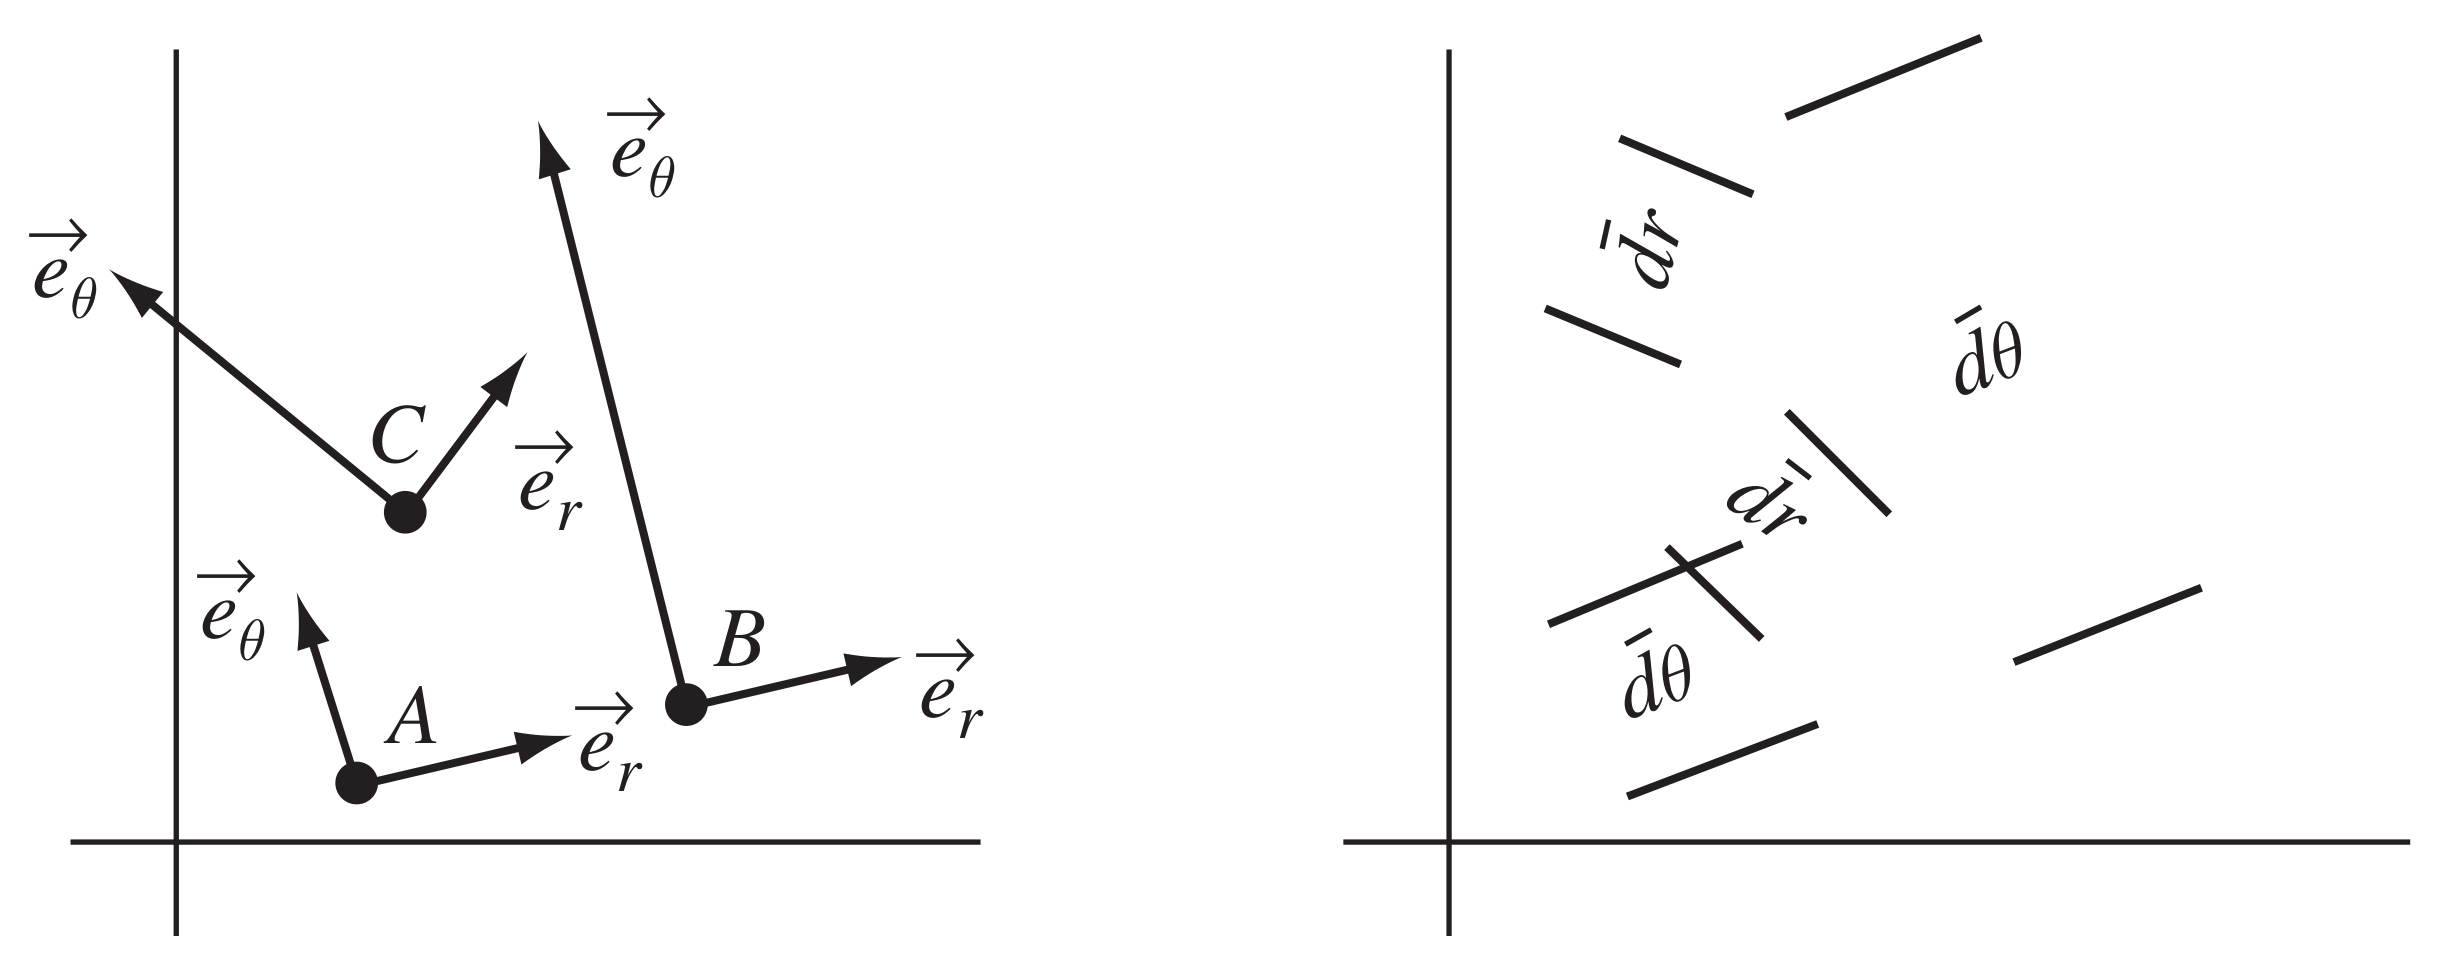
\includegraphics[width=0.7\textwidth]{fig5.5.png}
    \figcaption{极坐标系的向量基与1形式基图示}
    \label{fig5.5}
}

上面体现了一个非常重要的事实:各点的基互不相同。例如,图\ref{fig5.5}中$A$点与$C$点的向量基不平行。这是由于基向量指向坐标增加的方向,而这个方向随着点的改变而改变。此外,基的长度也不是恒定不变的。例如,根据\eqref{equ5.23}式可得

\begin{subequations}
\begin{alignat}{2}
    |\Ve_\theta|^2 &= \Ve_\theta \cdot \Ve_\theta = r^2 \sin^2 \theta + r^2 \cos^2 \theta = r^2,&& \label{equ5.28a} \\
    |\Ve_r| &= 1, \quad |\trd r| = 1, \quad |\trd \theta| = r^{-1}. &&\label{equ5.28b}
\end{alignat}
\end{subequations}
距离原点越远,$\Ve_\theta$的模长越大。因为$\Ve_\theta$在$(r, \theta)$系的分量为$(0, 1)$,意味着它表示$\theta$分量的1单位的位移,即1弧度。在半径更大的地方,移动1弧度的长度更大。因此极坐标基并非\textit{单位}基。其它基的模长容易求出。可以发现,$| \trd \theta|$在$r = 0$附近更大(更紧密),因为一个给定的向量在原点附近覆盖的$\theta$范围更大。

\subsection*{度规张量}
上面的点乘结果都是根据直角坐标系$x, y$中已知的度规来计算的:
\[
    \vec{e}_x \cdot \vec{e}_x = \vec{e}_y \cdot \vec{e}_y = 1, \quad \vec{e}_x \cdot \vec{e}_y = 0;
\]
或者用张量记号写为
\begin{equation}
    \mathbf{g} (\vec{e}_\alpha, \vec{e}_\beta) = \delta_{\alpha \beta} \quad \text{在直角坐标系中。}
\label{equ5.29}
\end{equation}
$\mathbf{g}$在极坐标系的分量是什么?根据分量的定义:
\begin{equation}
    g_{\alpha' \beta'} = \mathbf{g} (\vec{e}_{\alpha'}, \vec{e}_{\beta'}) = \vec{e}_{\alpha'} \cdot \vec{e}_{\beta'},
\label{equ5.30}
\end{equation}
或者根据\eqref{equ5.28}、\eqref{equ5.22}和\eqref{equ5.23}式可得
\begin{equation}
    g_{rr} = 1, \quad g_{\theta \theta} = r^2, \quad  g_{r \theta} = 0. \label{equ5.31}
\end{equation}
由此可得$\mathbf{g}$在极坐标系的分量为
\begin{equation}
    (g_{\alpha \beta})_{\text{polar}} = 
        \begin{pmatrix}
            1 & 0 \\
            0 & r^2
        \end{pmatrix},
\label{equ5.32}
\end{equation}
线元(line element)可以方便地同时表示$\mathbf{g}$的分量以及坐标,线元即为任意“无穷小”位移$\rd \vec{\ell}$的模:
\begin{shaded}
\begin{align}
    \rd \vec{\ell} \cdot \rd \vec{\ell} &= \rd s^2 = |\rd r \vec{e}_r + \rd \theta \vec{e}_\theta |^2 \notag \\
    &= \rd r^2 + r^2 \rd \theta^2. \label{equ5.33}
\end{align}
\end{shaded}
\textit{不要}将这里的$\rd r, \rd \theta$与1形式基$\trd r, \trd \theta$混淆,前者是$\rd \vec{\ell}$在极坐标系的分量,“$\rd$”就是“无穷小$\Delta$”的意思。 

另外有一种导出\eqref{equ5.33}式的方法值得一提。回顾\eqref{equ3.26}式,它表明任何$\binom{0}{2}$张量可以表示为$\binom{0}{2}$张量基$\trd x^\alpha \otimes \trd x^\beta$的线性组合:
\[
    \mathbf{g} = g_{\alpha \beta} \trd x^\alpha \otimes \trd x^\beta = \trd r \otimes \trd r + r^2 \trd \theta \otimes \trd \theta.
\]
尽管上式看起来像\eqref{equ5.33}式,但它们不一样:上式各项是算符,作用于向量$\rd \vec{\ell}$(其分量为$\rd r, \rd \theta$)之后得到\eqref{equ5.33}式。由于相应学科的符号混乱,导致上面两个式子非常不幸地十分相像。大多数教材与论文仍采用“旧式的”表达式——方程\eqref{equ5.33}来表示度规分量,本书遵从这一习惯。

度规分量矩阵存在逆矩阵:
\begin{equation}
    {\begin{pmatrix}
        1 & 0 \\
        0 & r^2
    \end{pmatrix} }^{-1} = 
    \begin{pmatrix}
        1 & 0 \\
        0 & r^{-2}
    \end{pmatrix}.
\label{equ5.34}
\end{equation}
由此可得$g^{rr} = 1, g^{r\theta} = 0, g^{\theta \theta} = 1/r^2$。这可以建立1形式与向量之间的映射。例如,向量场$\phi$的梯度场为$\trd \phi$,则这个1形式相应的向量$\rd \phi$具有分量
\begin{equation}
    (\vec{\rd} \phi)^\alpha = g^{\alpha \beta} \phi_{, \beta}
\label{equ5.35}
\end{equation}
或者写为
\begin{subequations}
\begin{alignat}{2}
    (\vec{\rd} \phi)^r &= g^{r \beta} \phi_{, \beta} = g^{rr} \phi_{, r} + g^{r \theta} \phi_{, \theta} \notag &&   \\
    &= \frac{\partial \phi}{\partial r}. &&\label{equ5.36a} \\
    (\vec{\rd} \phi)^\theta &= g^{\theta r} \phi_{, r} + g^{\theta \theta} \phi_{, \theta} && \notag \\
    &= \frac{1}{r^2} \frac{\partial \phi}{\partial \theta}. && \label{equ5.36b}
\end{alignat}
\end{subequations}
可见,1形式的分量是$(\phi_{, r}, \phi_{, \theta})$,而相应向量的分量是$(\phi_{, r}, \phi_{, \theta} / r^2)$。就算是在欧几里得空间,向量与相应的1形式的分量一般也不相同。直角坐标系是它们在其中唯一相等的坐标系。



\section{极坐标系的张量微积分}
\label{sec5.3}
极坐标系的基向量并非处处相等,这对向量求导产生了麻烦。例如,简单的直角坐标基$\vec{e}_x$,它在各点都相等,$\vec{e}_x$在极坐标系中的分量为$\vec{e}_x \to (\Lambda\indices{^r_x}, \Lambda\indices{^\theta_x}) = (\cos \theta, -r^{-1} \sin \theta)$。尽管$\vec{e}_x$处处相同,但显然它的分量不是常数,这是由于分量对应的基向量在各点不同。如果只把分量对坐标,例如对$\theta$求导,结果显然\textit{并非}$\partial \vec{e}_x / \partial \theta$,因为后者必须等于零。

从这个例子可见,对向量分量的求导结果一般情况下不是向量的导数,必须要考虑到基向量的变化。这是理解曲线坐标系与弯曲空间的关键。下面来系统讨论这些内容。

\subsection*{基向量的导数}
由于$\vec{e}_x$和$\vec{e}_y$是常向量场(在各点的值相同):
\begin{subequations}
\begin{alignat}{2}
    \frac{\partial}{\partial r} \vec{e}_r &= \frac{\partial}{\partial r} (\cos \theta \vec{e}_x + \sin \theta \vec{e}_y ) = 0,  &&\label{equ5.37a} \\
    \frac{\partial}{\partial \theta} \vec{e}_r &= \frac{\partial}{\partial \theta} (\cos \theta \vec{e}_x + \sin \theta \vec{e}_y) && \notag \\
    &= -\sin \theta \vec{e}_x + \cos \theta \vec{e}_y = \frac{1}{r} \vec{e}_\theta. && \label{equ5.37b}
\end{alignat}
\label{equ5.37}
\end{subequations}
这个结果有着简单的图像,如图\ref{fig5.6}。在相近的两点$A, B$,它们的$\vec{e}_r$的指向是从原点向外的径向,而有微小的差别。$\vec{e}_r$对$\theta$的导数就是$A, B$点的$\vec{e}_r$之差除以$\Delta \theta$。从图中可见,这个差平行于$\vec{e}_\theta$,这与方程\eqref{equ5.37b}相符。

{
    \centering
    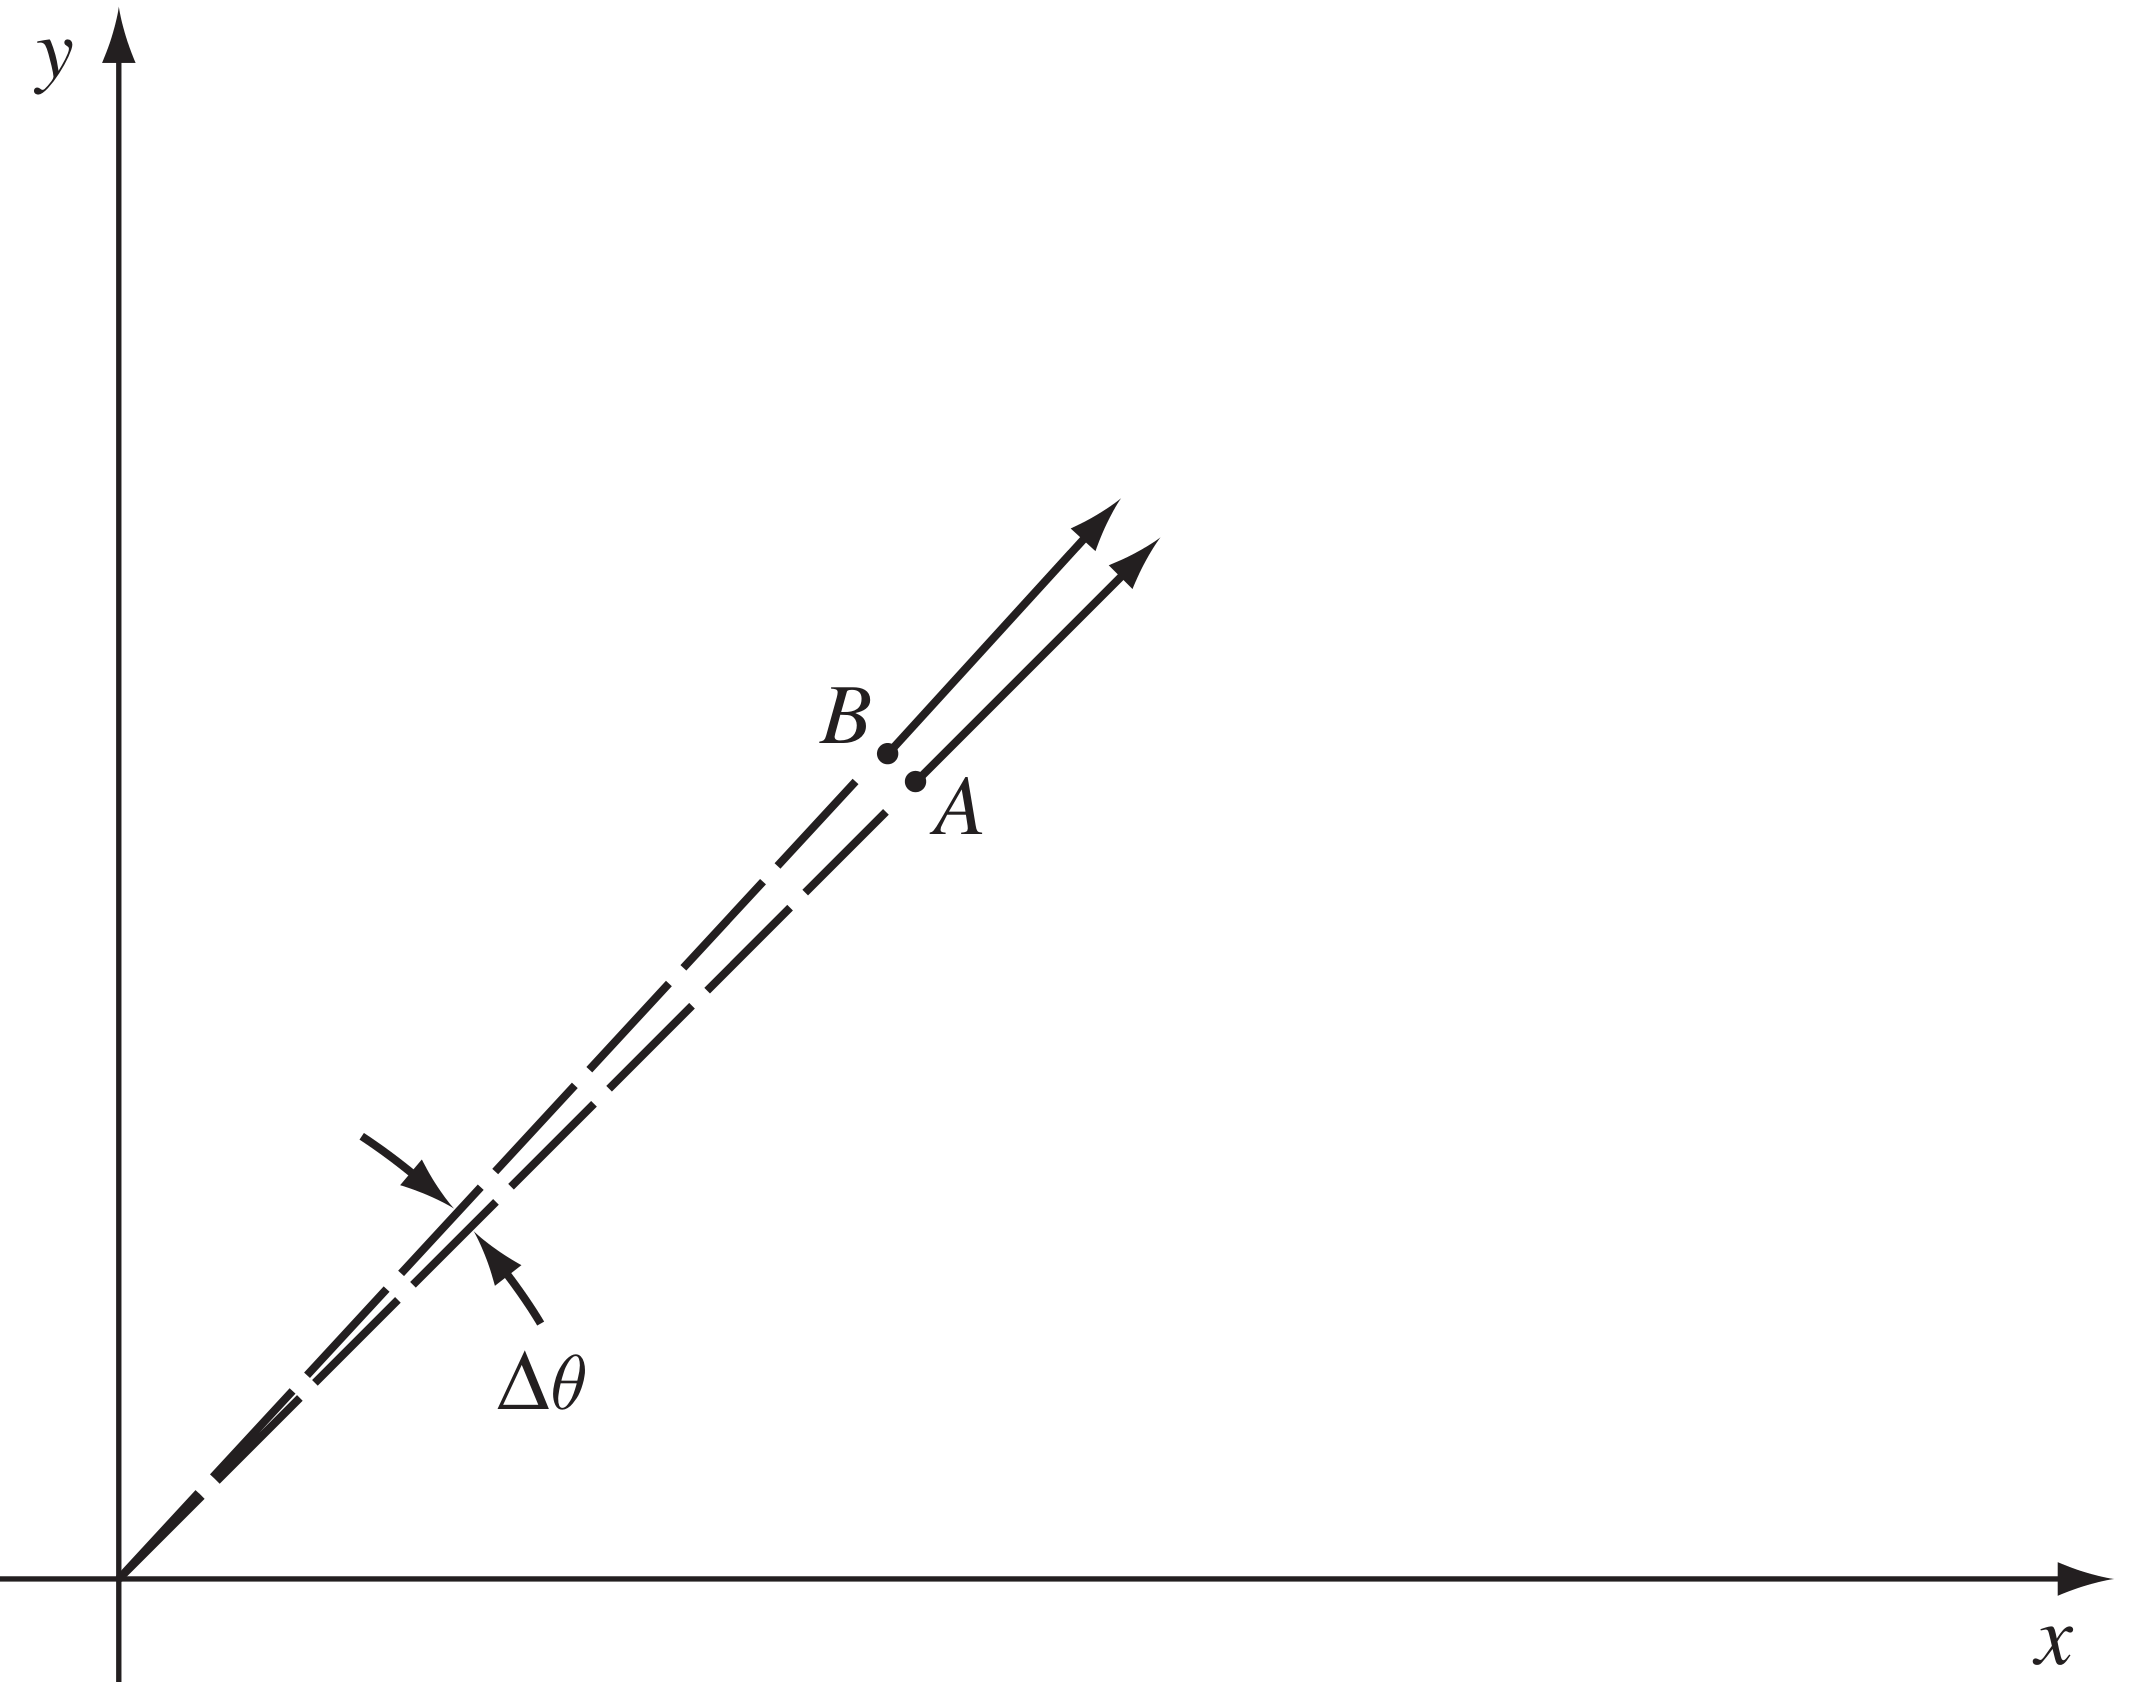
\includegraphics[width=0.65\textwidth]{fig5.6.png}
    \figcaption{\textit{$\theta$变化$\Delta \theta$造成的$\vec{e}_r$的变化。}}
    \label{fig5.6}
}

同理可得
\begin{subequations}
\begin{alignat}{2}
    \frac{\partial}{\partial r} \vec{e}_\theta &= \frac{\partial}{\partial r} (-r \sin \theta \vec{e}_x + r \cos \theta \vec{e}_y ) = 0, && \notag \\ 
    &= -\sin \theta \vec{e}_x + \cos \theta \vec{e}_y = \frac{1}{r} \vec{e}_\theta,  && \label{equ5.38a} \\
    \frac{\partial}{\partial \theta} \vec{e}_\theta &= -r \cos \theta \vec{e}_x - r \sin \theta \vec{e}_y = -r \vec{e}_r. && \label{equ5.38b}
\end{alignat}
\label{equ5.38}
\end{subequations}
米娜桑可以画类似\ref{fig5.6}那样的图来解释这些求导结果。

\subsection*{一般向量的导数}
回到$\vec{e}_x$的导数,既然
\begin{equation}
    \vec{e}_x = \cos \theta \vec{e}_r - \frac{1}{r} \sin \theta \vec{e}_\theta, 
\label{equ5.39}
\end{equation}
则有
\begin{align}
    \frac{\partial}{\partial \theta} \vec{e}_x =& \frac{\partial}{\partial \theta} (\cos \theta) \vec{e}_r + \cos \theta \frac{\partial}{\partial \theta} (\vec{e}_r) \notag \\
    & -\frac{\partial}{\partial \theta} \left( \frac{1}{r} \sin \theta \right) \vec{e}_\theta - \frac{1}{r} \sin \theta \frac{\partial}{\partial \theta} (\vec{e}_\theta) \label{equ5.40} \\
    =& -\sin \theta \vec{e}_r + \cos \theta \left( \frac{1}{r} \vec{e}_\theta \right) \notag \\
    & - \frac{1}{r} \cos \theta \vec{e}_\theta - \frac{1}{r} \sin \theta (-r \vec{e}_r). \label{equ5.41}
\end{align}
其中利用了\eqref{equ5.37}, \eqref{equ5.38}式。化简上式可得
\begin{equation}
    \frac{\partial}{\partial \theta} \vec{e}_x = 0,
\label{equ5.42}
\end{equation}
正如所料。\eqref{equ5.40}式中的第一、三项是$\vec{e}_x$的极坐标系分量的求导结果,另外两项是对极坐标系基向量的求导结果,它们彼此相消结果为零。

一般的向量$\vec{V}$在极坐标系的分量$(V^r, V^\theta)$,向量的导数,类比\eqref{equ5.40}式,等于:
\begin{align*}
    \frac{\partial \vec{V}}{\partial r} &= \frac{\partial}{\partial r} (V^r \vec{e}_r + V^\theta \vec{e}_\theta) \\
    &= \frac{\partial V^r}{\partial r} \vec{e}_r + V^r \frac{\partial \vec{e}_r}{\partial r} + \frac{\partial V^\theta}{\partial r} \vec{e}_\theta + V^\theta \frac{\partial \vec{e}_\theta}{\partial r},
\end{align*}
$\partial \vec{V} / \partial \theta$类似。上式用指标记号写为
\[
    \frac{\partial \vec{V}}{\partial r} = \frac{\partial}{\partial r} (V^\alpha \vec{e}_\alpha) = \frac{\partial V^\alpha}{\partial r} \vec{e}_\alpha + V^\alpha \frac{\partial \vec{e}_\alpha}{\partial r}.
\]
其中指标$\alpha$跑遍$r, \theta$。

由此可见,$\vec{V}$的导数不仅包括其分量$V^\alpha$的导数。$r$是坐标之一,上式对$r$的导数可以推广为对一般坐标的导数:
\begin{equation}
    \frac{\partial \vec{V}}{\partial x^\beta} = \frac{\partial V^\alpha}{\partial x^\beta} \vec{e}_\alpha + V^\alpha \frac{\partial \vec{e}_\alpha}{\partial x^\beta},
\label{equ5.43}
\end{equation}
其中$x^\beta, \beta = 1, 2$分别对应$r, \theta$。

\subsection*{Christoffel符号}
方程\eqref{equ5.43}的最后一项显然十分重要。由于$\partial \vec{e}_\alpha / \partial x^\beta$本身是个向量,它也可以表示为基向量的线性组合;线性组合的系数记作$\Gamma\indices{^\mu_{\alpha \beta}}$:
\begin{equation}
    \frac{\partial \vec{e}_\alpha}{\partial x^\beta} = \Gamma\indices{^\mu_{\alpha \beta}} \vec{e}_\mu.
\label{equ5.44}
\end{equation}
$\Gamma\indices{^\mu_{\alpha \beta}}$的含义是向量$\partial \vec{e}_\alpha / \partial x^\beta$的$\mu$分量。它有三个分量:一个分量($\alpha$)表明对哪个基向量求导;第二个($\beta$)表明基向量对哪个坐标求导;第三个($\mu$)表示求导结果向量的分量。$\Gamma\indices{^\mu_{\alpha \beta}}$十分有用,值得给它进行命名:称之为\textbf{Christoffel 符号}。Christoffel符号是不是张量的分量?这个问题之后讨论。

前面实际上已经算出了极坐标系的Christoffel,从方程\eqref{equ5.37}和\eqref{equ5.38}可得
\begin{equation}
\left.
\begin{split}
    (1)\ \ \dfrac{\partial \vec{e}_r}{\partial r} &= 0  \Rightarrow \Gamma\indices{^\mu_{rr}} = 0, \quad \forall\, \mu, \\
    (2)\ \  \dfrac{\partial \vec{e}_r}{\partial \theta} &= \dfrac{1}{r} \vec{e}_\theta \Rightarrow  \Gamma\indices{^r_{r\theta}} = 0, \quad \Gamma\indices{^\theta_{r \theta}} = \dfrac{1}{r}, \\
    (3)\ \  \dfrac{\partial \vec{e}_\theta}{\partial r} &= \dfrac{1}{r} \vec{e}_\theta \Rightarrow \Gamma\indices{^r_{\theta r}} = 0, \quad \Gamma\indices{^\theta_{\theta r}} = \dfrac{1}{r}, \\
    (4)\ \  \dfrac{\partial \vec{e}_\theta}{\partial \theta} &= -r \vec{e}_r \Rightarrow \Gamma\indices{^r_{\theta \theta}} = -r, \quad \Gamma\indices{^\theta_{\theta \theta}} = 0.
\end{split}
\right\}
\label{equ5.45}
\end{equation}
定义式\eqref{equ5.44}当中的所有指标都必须在同一个坐标系中。因此,尽管我们利用了$\vec{e}_x, \vec{e}_y$是常向量场的性质导出了$\vec{e}_r, \vec{e}_\theta$的导数,但是\eqref{equ5.45}中的各方程并不依赖直角坐标系。Christoffel符号的重要性在于,它可以将极坐标系基向量的导数只用极坐标系的量表示,而与其它坐标系无关。

\subsection*{协变导数}
利用Christoffel符号的定义\eqref{equ5.44}式,可以将\eqref{equ5.43}式的导数表示为
\begin{equation}
    \frac{\partial \vec{V}}{\partial x^\beta} = \frac{\partial V^\alpha}{\partial x^\beta} \vec{e}_\alpha + V^\alpha \Gamma\indices{^\mu_{\alpha \beta}} \vec{e}_\mu.
\label{equ5.46}
\end{equation}
最后一项表示了对傀儡指标$\alpha, \mu$的两个求和,对这两个傀儡指标重新命名:$\mu$换成$\alpha$,$\alpha$换成$\mu$得到
\begin{equation}
    \frac{\partial \vec{V}}{\partial x^\beta} = \frac{\partial V^\alpha}{\partial x^\beta} \vec{e}_\alpha + V^\mu \Gamma\indices{^\alpha_{\mu \beta}} \vec{e}_\alpha.
\label{equ5.47}
\end{equation}
这样重命名了傀标之后上式就可提出等号右侧的$\vec{e}_\alpha$项:
\begin{equation}
    \frac{\partial \vec{V}}{\partial x^\beta} = \left( \frac{\partial V^\alpha}{\partial x^\beta} + V^\mu \Gamma\indices{^\alpha_{\mu \beta}} \right) \vec{e}_\alpha.
\label{equ5.48}
\end{equation}
因此,向量场$\partial \vec{V} / \partial x^\beta$的分量为
\begin{equation}
    \frac{\partial V^\alpha}{\partial x^\beta} + V^\mu \Gamma\indices{^\alpha_{\mu \beta}}.
\label{equ5.49}
\end{equation}
回顾一下偏导数的简写记号:$\partial V^\alpha / \partial x^\beta = V\indices{^\alpha_{, \beta}}$,利用这个记号并定义一个\textit{新}记号:
\begin{shaded}
\begin{equation}
    V\indices{^\alpha_{; \beta}} := V\indices{^\alpha_{, \beta}} + V^\mu \Gamma\indices{^\alpha_{\mu \beta}}.
\label{equ5.50}
\end{equation}
\end{shaded}
在这个分号简写记号下:
\begin{shaded}
\begin{equation}
    \frac{\partial \vec{V}}{\partial x^\beta} = V\indices{^\alpha_{; \beta}} \vec{e}_\alpha
\label{equ5.51}
\end{equation}
\end{shaded}
它将\eqref{equ5.48}式表示成了非常紧凑的形式。

若将$\beta$视为固定不动的,则$\partial \vec{V} / \partial x^\beta$是个向量场。但是实际上$\beta$\textit{可以}有两种取值,所以$\partial \vec{V} / \partial x^\beta$可以视为将向量$\vec{e}_\beta$映为向量$\partial \vec{V} / \partial x^\beta$的$\binom{1}{1}$张量场,就像第\ref{chap3}章习题17那样。这个张量场称为$\vec{V}$的\textit{协变导数 (covariant derivative)},(很自然地)记作$\nabla \vec{V}$,它的分量为
\begin{equation}
    (\nabla \vec{V})\indices{^\alpha_\beta} = (\nabla_\beta \vec{V})\indices{^\alpha} = V\indices{^\alpha_{; \beta}} 
\label{equ5.52}
\end{equation}
在直角坐标系中,这些分量就等于$V\indices{^\alpha_{, \beta}}$。然而在曲线坐标系中,必须考虑基向量的导数,我们得到了$V\indices{^\alpha_{; \beta}}$是$\nabla \vec{V}$的分量,不论在哪个曲线坐标系,只要把那个系的Christoffel符号带入\eqref{equ5.50}式就能算出。上述内容的重要性不可低估,它是之后所有内容的基础。存在一个叫做$\nabla \vec{V}$的$\binom{1}{1}$张量,它在直角坐标系中的分量是$\partial V^\alpha / \partial x^\beta$,在一般的坐标系$\{ x^{\mu'} \}$中的分量是$V\indices{^{\alpha'}_{; \beta'}}$,这个分量可以通过两种方式计算:
\begin{itemize}
\item 直接在$\{ x^{\mu'} \}$坐标系中利用\eqref{equ5.50}式和那个系的Christoffel符号$\Gamma\indices{^{\alpha'}_{\mu' \beta'}}$计算;
\item 利用从直角坐标系到一般坐标系$\{ x^{\mu'} \}$的张量分量变换律计算。
\end{itemize}

标量的协变导数是啥?协变导数与普通偏导数的不同是由于基向量随着坐标变化。因为标量不依赖于基向量,因此标量的协变导数等于普通的偏导数,也就是梯度:
\begin{equation}
    \nabla_\alpha f = \frac{\partial f}{\partial x^\alpha}; \quad \nabla f = \trd f.
\label{equ5.53}
\end{equation}


\subsection*{散度,Laplacian}
在深入讨论之前,我们来研究一下与之前的内容有联系的部分。在直角坐标系中,向量$V^\alpha$的散度是$V\indices{^\alpha_{, \alpha}}$,它是由$V\indices{^\alpha_{, \beta}}$对上下指标缩并产生的标量。缩并是不依赖于坐标系的运算,因此$\vec{V}$的散度也可以在坐标系$\{ x^{\mu'} \}$中对$\nabla \vec{V}$的两个指标进行缩并得到,其结果为标量$V\indices{^{\alpha'}_{; \alpha'}}$,注意,它与直角坐标系中的$V\indices{^\alpha_{, \alpha}}$是\textbf{同一个量}:
\begin{equation}
    V\indices{^\alpha_{, \alpha}} \equiv V\indices{^{\beta'}_{; \beta'}}
\label{equ5.54}
\end{equation}
其中不带撇的指标表示直角坐标系,带撇的表示任意坐标系。

极坐标系(简明起见,用不带撇的指标表示)中:
\begin{equation*}
    V\indices{^\alpha_{; \alpha}} = \frac{\partial V^\alpha}{\partial x^\alpha} + \Gamma\indices{^\alpha_{\mu \alpha}} V_{\mu}.
\end{equation*}
根据\eqref{equ5.45}式可以算出:
\begin{equation}
\left.
\begin{split}
    \Gamma\indices{^\alpha_{r \alpha}} =& \Gamma\indices{^r_{rr}} + \Gamma\indices{^\theta_{r \theta}} = \frac{1}{r}, \\
    \Gamma\indices{^\alpha_{\theta \alpha}} =& \Gamma\indices{^r_{\theta r}} + \Gamma\indices{^\theta_{\theta \theta}} = 0.
\end{split}
\right\}
\label{equ5.55}
\end{equation}
从而
\begin{align}
    V\indices{^\alpha_{; \alpha}} =& \frac{\partial V^r}{\partial r} + \frac{\partial V^\theta}{\partial \theta} + \frac{1}{r} V^r, \notag \\
    =& \frac{1}{r} \frac{\partial}{\partial r} (r V^r) + \frac{\partial}{\partial \theta} V^\theta. \label{equ5.56}
\end{align}
上式看起来很面熟。更面熟的是梯度的散度,也就是Laplacian。但是散度是对向量定义的,而梯度是个1形式,因此必须先把1形式转换为向量。给定一个标量场$\phi$,根据\ref{sec5.2}节最后的\eqref{equ5.53}式可得,相应的梯度向量的分量为$(\phi_{, r},\ \phi_{, \theta} / r^2$。将它带入向量的散度公式\eqref{equ5.56}可得
\begin{equation}
    \nabla \cdot \nabla \phi := \nabla^2 \phi = \frac{1}{r} \frac{\partial}{\partial r} \left( r \frac{\partial \phi}{\partial r} \right) + \frac{1}{r^2} \frac{\partial^2 \phi}{\partial \theta^2}.
\label{equ5.57}
\end{equation}
这就是平面极坐标系中的Laplacian的表达式,它等同于
\begin{equation}
    \nabla^2 \phi = \frac{\partial^2 \phi}{\partial x^2} + \frac{\partial^2 \phi}{\partial y^2}.
\label{equ5.58}
\end{equation}



\subsection*{1形式与高阶张量的导数}
标量场$\phi$不依赖于基向量,它的导数$\trd \phi$与协变导数$\nabla \phi$相同,今后都采用符号$\trd \phi$。为了计算1形式的导数(和向量的导数一样并非仅仅是对分量求偏导数),我们利用1形式作用于向量得到标量的性质。设$\tilde{p}$是1形式,$\vec{V}$是向量,对于固定的指标$\beta$,$\nabla_\beta \tilde{p}$也是一个1形式,$\nabla_\beta \vec{V}$是向量,而$\langle \tilde{p}, \vec{V} \rangle \equiv \phi$是标量场,在任意坐标系中:
\begin{equation}
    \phi = p_\alpha V^\alpha.
\label{equ5.59}
\end{equation}
根据求导的乘积法则可以算出$\nabla_\beta \phi$:
\begin{equation}
    \nabla_\beta \phi = \phi_{, \beta} = \frac{\partial p_{\alpha}}{\partial x^\beta} V^\alpha + p_\alpha \frac{\partial V^\alpha}{\partial x^\beta}.
\label{equ5.60}
\end{equation}
利用方程\eqref{equ5.50}可以将$\partial V^\alpha / \partial x^\beta$用$V\indices{^\alpha_{; \beta}}$(即$\nabla_\beta \vec{V}$的分量)替换:
\begin{equation}
    \nabla_\beta \phi = \frac{\partial p_\alpha}{\partial x^\beta} V^\alpha + p_{\alpha} V\indices{^\alpha_{; \beta}} - p_\alpha V^\mu \Gamma\indices{^\alpha_{\mu \beta}}.
\label{equ5.61}
\end{equation}
重新安排各项,并且对Christoffel符号项的傀儡指标重命名可得:
\begin{equation}
    \nabla_\beta \phi = \left( \frac{\partial p_\alpha}{\partial x^\beta} - p_\mu \Gamma\indices{^\mu_{\alpha \beta}} \right) V^\alpha + p_\alpha V\indices{^\alpha_{; \beta}}
\label{equ5.62}
\end{equation}
对于任意向量$\vec{V}$,上式中括号之外的两项\textbf{都已知是}张量的分量,因此,由于张量分量的乘法加法得到的结果都是新张量,因此括号中的项也是张量分量,这就是1形式$\tilde{p}$的协变导数:
\begin{shaded}
\begin{equation}
    (\nabla_\beta \tilde{p})_\alpha := (\nabla \tilde{p})_{\alpha \beta} := p_{\alpha; \beta} = p_{\alpha, \beta} - p_\mu \Gamma\indices{^\mu_{\alpha \beta}}.
\label{equ5.63}
\end{equation}
\end{shaded}
这样,\eqref{equ5.62}式写为
\begin{shaded}
\begin{equation*}
    \nabla_\beta (p_\alpha V^\alpha) = p_{\alpha; \beta} V^\alpha + p_\alpha V\indices{^\alpha_{; \beta}}
\end{equation*}
\end{shaded}
可见协变导数也服从乘积法则,和\eqref{equ5.60}式一样。实际上\textbf{必须如此},因为在直角坐标系中$\nabla$就是偏导数算符,上式在直角坐标系中退化为\eqref{equ5.60}式。

比较向量与1形式的协变导数\eqref{equ5.50}和\eqref{equ5.63}式:
\begin{align*}
    V\indices{^\alpha_{; \beta}} =& V\indices{^\alpha_{, \beta}} + V^\mu \Gamma\indices{^\alpha_{\mu \beta}}, \\
    p_{\alpha; \beta} =& p_{\alpha, \beta} - p_\mu \Gamma\indices{^\mu_{\alpha \beta}}.
\end{align*}
它们有相似也有不同。只要记住求导的分量$\beta$总是$\Gamma$的\textbf{最后一个}指标,则其它指标的上下位置不难确定。还需要记住符号的不同,一个辅助的办法是记住$\Gamma\indices{^\alpha_{\mu \beta}}$与基向量的导数有关(因此是正号),而1形式基的导数就对应$-\Gamma\indices{^\alpha_{\mu \beta}}$,符号的不同意味着1形式基的变换规律与基向量“相反”,从而使得缩并$\langle \tilde{\omega}^\alpha, \vec{e}_\beta \rangle = \delta\indices{^\alpha_\beta}$在坐标变换下\textbf{不变},其导数为零。

高阶张量的协变导数与方程\eqref{equ5.63}的推导过程同理,这里只给出结果:
\begin{shaded}
\begin{align}
    \nabla_\beta T_{\mu \nu} =& T_{\mu \nu, \beta} - T_{\alpha \nu} \Gamma\indices{^\alpha_{\mu \beta}} - T_{\mu \alpha} \Gamma\indices{^\alpha_{\nu \beta}} ; \label{equ5.64} \\
    \nabla_\beta A^{\mu \nu} =& A\indices{^{\mu \nu}_{, \beta}} + A^{\alpha \nu} \Gamma\indices{^\mu_{\alpha \beta}} + A^{\mu \alpha} \Gamma\indices{^\nu_{\alpha \beta}}; \label{equ5.65} \\
    \nabla_\beta B\indices{^\mu_\nu} =& B\indices{^\mu_{\nu, \beta}} + B\indices{^\alpha_\nu} \Gamma\indices{^\mu_{\alpha \beta}} - B\indices{^\mu_\alpha} \Gamma\indices{^\alpha_{\nu \beta}}. \label{equ5.66}
\end{align}
\end{shaded}
仔细观察会发现它们是\textbf{很有规律的}。在普通导数之外的每一项都分配一个$\Gamma$,上指标就像向量、下指标就像1形式那样进行处理。\eqref{equ5.64}式的几何意义是,$\nabla_\beta T_{\mu \nu}$是$\binom{0}{3}$张量$\nabla \mathbf{T}$的分量,其中$\mathbf{T}$是$\binom{0}{2}$张量。类似地,\eqref{equ5.65}式中,$\mathbf{A}$是$\binom{2}{0}$张量而$\nabla \mathbf{A}$是$\binom{2}{1}$张量,其分量为$\nabla_\beta A^{\mu \nu}$。

\section{Christoffel符号与度规}
\label{sec5.4}
上面的关于协变导数的推导没有涉及度规张量的任何内容,但是由于度规将向量与1形式联系起来,因此这两者的协变导数之间必然有一些关系。在直角坐标系中,1形式与相应的向量分量\textbf{相等},而$\nabla$在该系中就是普通求导算符,因此1形式与向量分量的协变导数在直角坐标系中必然相等。这意味着任一向量$\vec{V}$及其相应的1形式$\tilde{V} = \mathbf{g} (\vec{V}, \ )$在直角坐标系中有:
\begin{equation}
    \nabla_\beta \tilde{V} = \mathbf{g} (\nabla_\beta \vec{V}, \ ).
\label{equ5.67}
\end{equation}
上式是张量方程,在\textbf{所有}坐标系都成立,由此导出
\begin{equation}
    V_{\alpha; \beta} = g_{\alpha \mu} V\indices{^\mu_{; \beta}}
\label{equ5.68}
\end{equation}
上式就是\eqref{equ5.67}式的分量形式。

上面的论述也许不让你满意,下面一步一步重新推导一遍。用不带撇的指标$\alpha, \beta, \gamma, \dots$表示直角坐标系,带撇指标$\alpha', \beta', \gamma', \dots$表示\textbf{任意}坐标系。

我们的出发点是,在任意坐标系中,1形式与向量分量的对应关系为:
\begin{equation}
    V_{\alpha'} = g_{\alpha' \mu'} V^{\mu'}.
\label{equ5.69}
\end{equation}
而在直角坐标系中:
\begin{equation*}
    g_{\alpha \mu} = \delta_{\alpha \mu}, \quad V_{\alpha} = V^\alpha.
\end{equation*}
在直角坐标系中,Christoffel符号为零,因此在其中
\begin{equation*}
    V_{\alpha; \beta} = V_{\alpha, \beta}\quad V\indices{^\alpha_{; \beta}} = V\indices{^\alpha_{, \beta}}
\end{equation*}
由此可得
\[
    V_{\alpha; \beta} = V\indices{^\alpha_{; \beta}}
\]
这只在直角坐标系成立。为了将上式写成在任意坐标系都成立的形式,我们注意到在直角坐标系中
\begin{equation*}
    V\indices{^\alpha_{; \beta}} = g_{\alpha \mu} V\indices{^\mu_{; \beta}}
\end{equation*}
由上两式可得
\[
    V_{\alpha; \beta} = g_{\alpha \mu} V\indices{^\mu_{; \beta}}
\]
这就写成了张量方程,在所有坐标系成立,于是再次得到了\eqref{equ5.68}式:
\begin{equation}
    V_{\alpha'; \beta'} = g_{\alpha' \mu'} V\indices{^{\mu'}_{; \beta'}}
\label{equ5.70}
\end{equation}
上式有个重要推论。方程\eqref{equ5.69}对$\beta'$坐标求协变导数可得
\[
    V_{\alpha'; \beta'} = g_{\alpha' \mu'; \beta'} V^{\mu'} + g_{\alpha' \mu'} V\indices{^{\mu'}_{; \beta'}}    
\]
上式与\eqref{equ5.70}式比较(注意$\vec{V}$是任意向量)可得
\begin{shaded}
\begin{equation}
    g_{\alpha' \mu'; \beta'} \equiv 0,
\label{equ5.71}
\end{equation}
\end{shaded}
上式在任意坐标系都成立,它是方程\eqref{equ5.67}的推论,在直角坐标系中
\[
    g_{\alpha \mu; \beta} \equiv g_{\alpha \mu, \beta} = \delta_{\alpha \mu, \beta} = 0,
\]
它是个平凡的恒等式。而在一般坐标系中,度规的协变导数为零是不显然的,下面以极坐标系为例计算一下以验证结论是否正确。

利用\eqref{equ5.64}式可得(以下不带撇指标表示一般坐标系)
\begin{equation}
    g_{\alpha \beta; \mu} = g_{\alpha \beta, \mu} - \Gamma\indices{^\nu_{\alpha \mu}} g_{\nu \beta} - \Gamma\indices{^\nu_{\beta \mu}} g_{\alpha \nu}.
\label{equ5.72}
\end{equation}
在极坐标系中,考虑分量$\alpha = r, \beta = r, \mu = r$:
\[
    g_{rr; r} = g_{rr, r} - \Gamma\indices{^\nu_{rr}} g_{\nu r} - \Gamma\indices{^\nu_{rr}} g_{r \nu}.
\]
由于$g_{rr, r} = 0, \Gamma\indices{^\nu_{rr}} = 0, \forall\, \nu$,因此上式平淡地等于零。对于分量$\alpha = \theta, \beta = \theta, \mu = r$就不那么平淡了:
\[
    g_{\theta \theta; r} = g_{\theta \theta, r} - \Gamma\indices{^\nu_{\theta r}} g_{\nu \theta} - \Gamma\indices{^\nu_{\theta r}} g_{\theta \nu}.
\]
带入$g_{\theta \theta} = r^2, \Gamma\indices{^\theta_{\theta r}} = 1/r, \Gamma\indices{^r_{\theta r}} = 0$可得
\[
    g_{\theta \theta; r} = (r^2)_{, r} - \frac{1}{r} (r^2) - \frac{1}{r} (r^2) = 0.
\]
就像某种魔法让它等于零一样,但是这不是魔法,只是因为在直角坐标系中$g_{\alpha \beta, \mu} = 0$,而在任意坐标系中的$g_{\alpha \beta; \mu}$与$g_{\alpha \beta, \mu}$是\textbf{同一}张量$\nabla \mathbf{g}$在不同坐标系的分量。

现在应该总结一下我们干了些什么。利用欧几里得空间中平行的概念,我们引入了协变微分,然后证明了欧几里得空间的度规是协变不变的(\eqref{equ5.71}式)。之后讨论弯曲空间(Riemannian空间)的时候需要更仔细地研究平行,但是在那里\eqref{equ5.71}式\textbf{仍然有效},因此以该方程为基础的所有讨论内容也依然有效。

\subsection*{从度规计算Christoffel符号}
\eqref{equ5.72}式等于零有一个极其重要的推论,下面会看到,利用\eqref{equ5.72}式可以用$\Gamma\indices{^\mu_{\alpha \beta}}$表示$g_{\alpha \beta, \mu}$,而反过来也可以,即用$g_{\alpha \beta, \mu}$表示$\Gamma\indices{^\mu_{\alpha \beta}}$,这是计算Christoffel符号的简单方式。

为此,先得证明一个重要命题:\textbf{在任意坐标系中}$\Gamma\indices{^\mu_{\alpha \beta}} \equiv \Gamma\indices{^\mu_{\beta \alpha}}$。为了证明这一对称性,考虑任意张量场$\phi$,它的一阶导数$\nabla \phi$是分量为$\phi_{, \beta}$的1形式,它的二阶导数——$\binom{0}{2}$张量$\nabla \nabla \phi$的分量为$\phi_{, \beta; \alpha}$,在直角坐标系中,这些分量等于
\[
    \phi_{, \beta, \alpha} := \frac{\partial}{\partial x^\alpha} \frac{\partial}{\partial x^\beta} \phi,
\]
它的$\alpha, \beta$指标是对称的,因为偏导数互相对易。如果张量在一个坐标系中的指标对称,则在任意坐标系中的指标都对称。因此
\begin{equation}
    \phi_{, \beta; \alpha} = \phi_{, \alpha; \beta}
\label{equ5.73}
\end{equation}
在\textbf{任意}坐标系成立,根据定义式\eqref{equ5.63}将上式展开:
\[
    \phi_{, \beta, \alpha} - \phi_{, \mu} \Gamma\indices{^\mu_{\beta \alpha}} = \phi_{, \alpha, \beta} - \phi_{, \mu} \Gamma\indices{^\mu_{\alpha \beta}} \quad \text{在任意坐标系中。}
\]
而在\textbf{任意}坐标系中都有
\[
    \phi_{, \alpha, \beta} = \phi_{,\beta ,\alpha}
\]
由此可得
\[
    \Gamma\indices{^\mu_{\alpha \beta}} \phi_{, \mu} = \Gamma\indices{^\mu_{\beta \alpha}} \phi_{, \mu}
\]
对任意标量场$\phi$成立,这就证明了在任意坐标系中Christoffel符号的对称性:
\begin{shaded}
\begin{equation}
    \Gamma\indices{^\mu_{\alpha \beta}} = \Gamma\indices{^\mu_{\beta \alpha}}.
\label{equ5.74}
\end{equation}
\end{shaded}
利用上式与\eqref{equ5.72}式,进行一些指标上的旋转跳跃就能得到\eqref{equ5.72}式的逆形式,将方程\eqref{equ5.72}进行指标轮换:
\begin{align*}
    g_{\alpha \beta, \mu} =& \Gamma\indices{^\nu_{\alpha \mu}} g_{\nu \beta} + \Gamma\indices{^\nu_{\beta \mu}} g_{\alpha \nu}, \\
    g_{\alpha \mu, \beta} =& \Gamma\indices{^\nu_{\alpha \beta}} g_{\nu \mu} + \Gamma\indices{^\nu_{\mu \beta}} g_{\alpha \nu}, \\
    -g_{\beta \nu, \alpha} =& -\Gamma\indices{^\nu_{\beta \alpha}} g_{\nu \mu} - \Gamma\indices{^\nu_{\mu \alpha}} g_{\beta \nu}.
\end{align*}
以上三式相加,并利用$\mathbf{g}$的对称性$g_{\beta \nu} = g_{\nu \beta}$合并同类项:
\begin{align*}
    g_{\alpha \beta, \mu} +& g_{\alpha \mu, \beta} - g_{\beta \mu, \alpha} \\
    =& (\Gamma\indices{^\nu_{\alpha \mu}} - \Gamma\indices{^\nu_{\mu \alpha}}) g_{\nu \beta} + ( \Gamma\indices{^\nu_{\alpha \beta}} - \Gamma\indices{^\nu_{\beta \alpha}} ) g_{\nu \mu} + ( \Gamma\indices{^\nu_{\beta \mu}} + \Gamma\indices{^\nu_{\mu \beta}} ) g_{\alpha \nu}.
\end{align*}
根据$\Gamma$的对称性$\eqref{equ5.74}$式,上式右侧前两项为零,于是
\[
    g_{\alpha \beta, \mu} + g_{\alpha \mu, \beta} - g_{\beta \mu, \alpha} = 2 g_{\alpha \nu} \Gamma\indices{^\nu_{\beta \mu}}.
\]
就快要完成了。上式左右两边除以2,乘以$g^{\alpha \gamma}$(重复指标$\alpha$表示求和),并且利用
\[
    g^{\alpha \gamma} g_{\alpha \nu} \equiv \delta\indices{^\gamma_\nu}
\]
可得
\begin{shaded}
\begin{equation}
    \frac{1}{2} g^{\alpha \gamma} (g_{\alpha \beta, \mu} + g_{\alpha \mu, \beta} - g_{\beta \mu, \alpha}  ) = \Gamma\indices{^\gamma_{\beta \mu}}.
\label{equ5.75}
\end{equation}
\end{shaded}
这就是利用度规$\mathbf{g}$的分量及其导数表示Christoffel符号的表达式。例如,在极坐标系中:
\[
    \Gamma\indices{^\theta_{r \theta}} = \frac{1}{2} g^{\alpha \theta} (g_{\alpha r, \theta} + g_{\alpha \theta, r} - g_{r \theta, \alpha}).
\]
由于$g^{r \theta} = 0$以及$g^{\theta \theta} = r^{-2}$,可以导出
\begin{align*}
    \Gamma\indices{^\theta_{r \theta}} =& \frac{1}{2r^2} (g_{\theta r, \theta} + g_{\theta \theta, r} - g_{r \theta, \theta}) \\
    =& \frac{1}{2r^2} g_{\theta \theta, r} = \frac{1}{2r^2} (r^2)_{, r} = \frac{1}{r}.
\end{align*}
这与前面推导的结果相同。这种计算Christoffel符号的方法是坠吼的,方程\eqref{equ5.75}值得记住。尽管是在欧几里得空间推导的,但之后会看到它在弯曲空间中同样有效。


\subsection*{$\Gamma\indices{^\alpha_{\beta \mu}}$的张量性}
$\vec{e}_\alpha$是个向量,$\nabla \vec{e}_\alpha$是个$\binom{1}{1}$张量,它的分量是$\Gamma\indices{^\mu_{\alpha \beta}}$,这里的$\alpha$固定而$\mu, \beta$是分量指标:$\alpha$变化对应不同的张量$\nabla \vec{e}_\alpha$,而改变$\mu$或$\beta$只是对应同一张量的不同分量。

因此,可以把$\mu, \beta$视为分量指标,而把$\alpha$视为指明不同张量的标签,每个基向量$\vec{e}_\alpha$对应这样一个张量。然而这不太有用,因为在坐标变换之下,新旧坐标系的基向量不同,在新坐标系中重要的张量是\textbf{新的}$\nabla \vec{e}_{\beta'}$,它与旧的$\nabla \vec{e}_\alpha$的关系很复杂:它们是\textbf{不同的}张量,而非同一张量在不同坐标系的分量。因此一个坐标系中的$\Gamma\indices{^\mu_{\alpha \beta}}$不能由另一坐标系的$\Gamma\indices{^{\mu'}_{\alpha'
 \beta'}}$经过简单的变换得到。最简单的例子是在直角坐标系中所有的$\Gamma$都为零,而在一般的坐标系中非零。因此很多教材都说$\Gamma\indices{^\mu_{\alpha \beta}}$不是张量分量。从我们的观点来看,这话并不严格正确:$\Gamma\indices{^\mu_{\alpha \beta}}$是\textbf{一组}$\binom{1}{1}$\textbf{张量}$\nabla \vec{e}_\alpha$的$(\mu, \beta)$分量,只是不存在一个$\binom{1}{2}$张量的分量是$\Gamma\indices{^\mu_{\alpha \beta}}$,因此形如$\Gamma\indices{^\mu_{\alpha \beta}} V^\alpha $的表达式也不是单个张量的分量,而组合
 \[
    V\indices{^\beta_{, \alpha}} + V^\mu \Gamma\indices{^\beta_{\mu \alpha}}
\]
\textbf{是}张量$\nabla \vec{V}$的分量。



\section{非坐标基}
\label{sec5.5}
之前所有的讨论都默认了非直角坐标系的基向量是由直角坐标$(x, y)$变换为某个$(\xi, \eta)$产生的。然而,下面会看到,并非所有基向量场都可以通过这种方式得到,并且我们要研究需要什么条件(不多)才可以。本书几乎不适用非坐标基,但是在平坦空间曲线坐标系的标准教材中却经常使用它们,因此有必要对它们进行介绍。

\subsection*{极坐标基}
极坐标系的基向量的定义是
\[
    \vec{e}_{\alpha'} = \Lambda\indices{^\beta_{\alpha'}} \vec{e}_{\beta},
\]
其中带撇指标表示极坐标,不带撇的表示直角坐标。此外,
\[
    \Lambda\indices{^\beta_{\alpha'}} = \frac{\partial x^\beta}{\partial x^{\alpha'}},
\]
这里将直角坐标$\{ x^\beta \}$视为极坐标$\{  x^{\alpha'} \}$的函数。可以导出
\[
    \vec{e}_{\alpha'} \cdot \vec{e}_{\beta'} \equiv g_{\alpha' \beta'} \neq \delta_{\alpha' \beta'},
\]
这意味着极坐标系\textbf{并非}单位向量。

\subsection*{极坐标单位基}
便利起见,经常定义\textbf{单位}基向量。容易导出极坐标系的单位基向量为:
\begin{equation}
    \vec{e}_{\hat{r}} = \vec{e}_{r}, \quad \vec{e}_{\hat{\theta}} = \frac{1}{r} \vec{e}_\theta,
\label{equ5.76}
\end{equation}
相应的1形式基为
\begin{equation}
    \tilde{\omega}^{\hat{r}} = \trd r, \quad \tilde{\omega}^{\hat{\theta}} = r \trd \theta.
\label{equ5.77}
\end{equation}
米娜桑应该自行证明
\begin{equation}
\left.
\begin{split}
    \vec{e}_{\hat{\alpha}} \cdot \vec{e}_{\hat{\beta}} \equiv g_{\hat{\alpha} \hat{\beta}} = \delta_{\hat{\alpha} \hat{\beta}}, \\
    \tilde{\omega}^{\hat{\alpha}} \cdot \tilde{\omega}^{\hat{\beta}} \equiv g^{\hat{\alpha} \hat{\beta}} = \delta^{\hat{\alpha} \hat{\beta}}.
\end{split}
\right\}
\label{equ5.78}
\end{equation}
这样就定义了正交归一的向量与1形式基,用带帽号$\hat{\ }$的指标表示。现在问题来了,是否存在坐标系$(\xi, \eta)$使得
\begin{subequations}
\begin{alignat}{2}
    \vec{e}_{\hat{\alpha}} =& \vec{e}_\xi = \frac{\partial x}{\partial \xi} \vec{e}_x + \frac{\partial y}{\partial \xi} \vec{e}_y  && \label{equ5.79a} \\
    \vec{e}_{\hat{\theta}} =& \vec{e}_\eta = \frac{\partial x}{\partial \eta} \vec{e}_x + \frac{\partial y}{\partial \eta} \vec{e}_y &&\label{equ5.79b}
\end{alignat}
\end{subequations}
成立?

如果成立,则$\{ \vec{e}_{\hat{\alpha}}, \vec{e}_{\hat{\theta}} \}$就是坐标系$(\xi, \eta)$的基向量,可以称之为坐标基;如果证明满足条件的$(\xi, \eta)$不存在,则这些向量是非坐标基。用相应的1形式基证明会更加容易,因此,下面要尝试找到坐标系$(\xi, \eta)$使得
\begin{equation}
\left.
\begin{split}
    \tilde{\omega}^{\hat{r}} =& \trd \xi = \frac{\partial \xi}{\partial x} \trd x + \frac{\partial \xi}{\partial y} \trd y, \\
    \tilde{\omega}^{\hat{\theta}} =& \trd \eta = \frac{\partial \eta}{\partial x} \trd x + \frac{\partial \eta}{\partial y} \trd y.
\end{split}
\right\}
\label{equ5.80}
\end{equation}
$\tilde{\omega}^{\hat{r}}, \tilde{\omega}^{\hat{\theta}}$关于$\trd r, \trd \theta$的关系已知,因此根据\eqref{equ5.26}和\eqref{equ5.27}式可得
\begin{equation}
\left.
\begin{split}
    \tilde{\omega}^{\hat{r}} =& \trd r = \cos \theta \trd x + \sin \theta \trd y, \\
    \tilde{\omega}^{\hat{\theta}} =& r \trd \theta = -\sin \theta \trd x + \cos \theta \trd y.
\end{split}
\right\}
\label{equ5.81}
\end{equation}
(不难验证$\tilde{\omega}^{\hat{r}}, \tilde{\omega}^{\hat{\theta}}$是正交的)

如果$(\xi, \theta)$存在,则
\begin{equation}
    \frac{\partial \eta}{\partial x} = -\sin \theta, \quad \frac{\partial \eta}{\partial y} = \cos \theta.
\label{equ5.82}
\end{equation}
如果上式成立,则混合导数相等:
\begin{equation}
    \frac{\partial}{\partial y} \frac{\partial \eta}{\partial x} = \frac{\partial}{\partial x} \frac{\partial \eta}{\partial y}.
\label{equ5.83}
\end{equation}
这意味着
\begin{equation}
    \frac{\partial}{\partial y} (-\sin \theta) = \frac{\partial}{\partial x} (\cos \theta)
\label{equ5.84}
\end{equation}
也就是
\begin{equation*}
    \frac{\partial}{\partial y} \left( \frac{y}{\sqrt{x^2 + y^2}} \right) + \frac{\partial}{\partial x} \left( \frac{x}{\sqrt{x^2 + y^2}} \right)  = 0.
\end{equation*}
上式当然\textbf{不可能成立}。因此$\xi, \eta$\textbf{不存在}:无法找到符合条件的坐标系。(If this manner of proof is surprising, try it on $\trd r$ and $\trd \theta$ themselves.)

关于曲线坐标系中向量微积分的教材几乎都采用正交归一基,而非坐标基。例如,某个向量在极坐标系\textbf{坐标基}(coordinate basis, PC)下的分量为
\begin{equation}
    \vec{V} \xrightarrow[\text{PC}]{ } (a, b) = \{ V^{\alpha'} \},
\label{equ5.85}
\end{equation}
则它在\textbf{正交基} (orthonormal basis, PO)下的分量为:
\begin{equation}
    \Vec{V} \xrightarrow[\text{PO}]{ } (a, rb) = \{ V^{\hat{\alpha}} \}.
\label{equ5.86}
\end{equation}
例如,相关教材计算向量散度的公式为:(与我们导出的\eqref{equ5.56}式有所不同)
\begin{equation}
    \nabla \cdot \mathbf{V} = \frac{1}{r} \frac{\partial}{\partial r} (r V^{\hat{r}}) + \frac{1}{r} \frac{\partial}{\partial \theta} V^{\hat{\theta}}.
\label{equ5.87}
\end{equation}
\eqref{equ5.56}和\eqref{equ5.87}式的不同只是因为$\Vec{V}$的基向量不同。

\subsection*{非坐标基总论}
坐标基与非坐标基的主要区别是啥?考虑任意标量场$\phi$,$\vec{e}_\mu$是任意一组基当中的基向量,$\trd \phi (\vec{e}_\mu)$是个标量,它可以记作
\begin{equation}
    \trd \phi (\vec{e}_\mu) = \phi_{,\mu}
\label{equ5.88}
\end{equation}
如果$\vec{e}_\mu$是坐标基的一员,则$\trd \phi (\vec{e}_\mu) = \partial \phi / \partial x^\mu$,并且在之前的章节中定义过:
\begin{equation}
    \phi_{, \mu} = \frac{\partial \phi}{\partial x^\mu}: \quad \text{对坐标基成立。}
\label{equ5.89}
\end{equation}
但是,如果$\vec{e}_\mu$是非坐标基,则\eqref{equ5.89}式必然失效。如果用方程\eqref{equ5.88}来\textbf{定义} $\phi_{,\hat{\mu}}$,例如对极坐标单位基$\vec{e}_{\hat{\theta}} = \vec{e}_{\theta} / r$有
\begin{equation}
    \phi_{, \hat{\theta}} = \frac{1}{r} \frac{\partial \phi}{\partial \theta}.
\label{equ5.90}
\end{equation}
一般情况下,对任意坐标系$\{ x^\beta \}$与非坐标基$\{ \vec{e}_{\hat{\alpha}} \}$有
\begin{equation}
    \nabla_{\hat{\alpha}} \phi \equiv \phi_{, \hat{\alpha}} = \Lambda\indices{^\beta_{\hat{\alpha}}} \nabla_\beta \phi = \Lambda\indices{^\beta_{\hat{\alpha}}} \frac{\partial \phi}{\partial x^\beta}
\label{equ5.91}
\end{equation}
因此按照\eqref{equ5.88}式的记号定义是很方便的,而$\phi_{, \mu} = \partial \phi / \partial x^\mu$只对坐标基成立。

对于非坐标基,Christoffel符号仿照之前的定义:
\begin{equation}
    \nabla_{\hat{\beta}} \vec{e}_{\hat{\alpha}} = \Gamma\indices{^{\hat{\mu}}_{\hat{\alpha} \hat{\beta}}} \vec{e}_{\hat{\mu}},
\label{equ5.92}
\end{equation}
只是协变导数的定义变成了
\begin{equation}
    \nabla_{\hat{\beta}} = \Lambda\indices{^\alpha_{\hat{\beta}}} \frac{\partial}{\partial x^\alpha},
\label{equ5.93}
\end{equation}
其中$\{x^\alpha\}$是任意坐标系,$\{ \vec{e}_{\hat{\beta}} \}$是任意基(坐标基或非坐标基)。然而\textbf{不能证明}$\Gamma\indices{^{\hat{\mu}}_{\hat{\alpha} \hat{\beta}}} = \Gamma\indices{^{\hat{\mu}}_{\hat{\beta} \hat{\alpha}}}$,因为证明过程要用到$\phi_{,\hat{\alpha} ,\hat{\beta}} = \phi_{,\hat{\beta} ,\hat{\alpha}}$,这只对坐标基才成立(偏导数互相对易)。因此,用$g_{\alpha \beta, \gamma}$表示$\Gamma\indices{^\mu_{\alpha \beta}}$的\eqref{equ5.75}式也只对坐标基成立。一般的表达式在第\ref{chap5}章习题20推导。

非坐标基不存在对应坐标系的一般原因是什么?设$\{ \tilde{\omega}^{\bar{\alpha}} \}$是坐标1形式基,它与另一组1形式基$\{ \trd x^\alpha \}$的关系为
\begin{equation}
    \tilde{\omega}^{\bar{\alpha}} = \Lambda\indices{^{\bar{\alpha}}_\beta} \trd x^\beta = \frac{\partial x^{\bar{\alpha}}}{\partial x^\beta} \trd x^\beta.
\label{equ5.94}
\end{equation}
关键在于$\Lambda\indices{^{\bar{\alpha}}_\beta}$,它是坐标的函数,而且是偏导数$\partial x^{\bar{\alpha}} / \partial x^\beta$,因此根据混合偏导数不依赖求导次序可得
\begin{equation}
    \frac{\partial}{\partial x^\gamma} \Lambda\indices{^{\bar{\alpha}}_\beta} = \frac{\partial^2 x^{\bar{\alpha}}}{\partial x^\gamma \partial x^\beta} = \frac{\partial^2 x^{\bar{\alpha}}}{\partial x^\beta \partial x^\gamma} = \frac{\partial}{\partial x^\beta} \Lambda\indices{^{\bar{\alpha}}_\gamma}.
\label{equ5.95}
\end{equation}
上式称为“可积性条件(integrability conditions)”,如果$\tilde{\omega}^{\bar{\alpha}}$是坐标基,则所有的变换矩阵元$\Lambda\indices{^{\bar{\alpha}}_\beta}$都要满足上式。显然,总可以构造不满足上式的变换矩阵,从而生成非坐标基。


\subsection*{本书的非坐标基}
我们几乎不会用到非坐标基,只要清楚理解存在非坐标基、并非所有基向量都可以从坐标系导出就行了。坐标基的代数运算几乎总是更简单。

那么,为啥向量分析的标准教材在讲述曲线坐标系的时候总是采用正交基呢?因为那是以欧几里得空间为背景的,度规分量是$\delta_{\alpha \beta}$,因此点乘的简单形式、向量与1形式的分量相等这些好的性质直接来自于直角坐标系(它是\textbf{唯一的}正交坐标基!)。为了在向量与张量微积分中利用坐标基的简单性,我们在前面花了大量时间学习了向量与1形式的不同!

\section{展望下一步}
\label{sec5.6}
这一章讨论了后面研究弯曲空间与时空的几乎所有符号和概念。\ref{sec5.2}-\ref{sec5.4}节特别重要,因为后面会仿照这些内容建立描述曲率的数学工具,读者务必精读这几节。下一步要添加的内容是关于平行的进一步讨论,以及计量欧几里得平行公理在弯曲空间的失效程度,进行计量的数学工具就是著名的Riemann张量。

\section{扩展阅读}
\label{sec5.7}
Dicke (1964), Misner et al. (1973), Shapiro (1980),
and Will (1993, 2006)讨论了Eötvös与Pound–Rebka–Snider实验以及其它验证GR的实验。Hoffmann(1983)用较少的数学讨论引入了曲率。Ashby (2003) 提供了最新的关于相对论在GPS系统应用的综述。

如下文献从不同方面建立了曲线坐标系的数学工具:Abraham and Marsden (1978), Lovelock and Rund (1990), and Schutz (1980b).

\section{习题}
\label{sec5.8}